\documentclass[12pt,]{article}
\usepackage{lmodern}
\usepackage{amssymb,amsmath}
\usepackage{ifxetex,ifluatex}
\usepackage{fixltx2e} % provides \textsubscript
\ifnum 0\ifxetex 1\fi\ifluatex 1\fi=0 % if pdftex
  \usepackage[T1]{fontenc}
  \usepackage[utf8]{inputenc}
\else % if luatex or xelatex
  \ifxetex
    \usepackage{mathspec}
  \else
    \usepackage{fontspec}
  \fi
  \defaultfontfeatures{Ligatures=TeX,Scale=MatchLowercase}
\fi
% use upquote if available, for straight quotes in verbatim environments
\IfFileExists{upquote.sty}{\usepackage{upquote}}{}
% use microtype if available
\IfFileExists{microtype.sty}{%
\usepackage{microtype}
\UseMicrotypeSet[protrusion]{basicmath} % disable protrusion for tt fonts
}{}
\usepackage[margin=1in]{geometry}
\usepackage{hyperref}
\PassOptionsToPackage{usenames,dvipsnames}{color} % color is loaded by hyperref
\hypersetup{unicode=true,
            pdfkeywords={Recurrent Neural Networks, Machine Learning, Data Science, Probabilistic
Sequence Generation, Sentiment Analysis},
            colorlinks=true,
            linkcolor=red,
            citecolor=Blue,
            urlcolor=red,
            breaklinks=true}
\urlstyle{same}  % don't use monospace font for urls
\usepackage{graphicx,grffile}
\makeatletter
\def\maxwidth{\ifdim\Gin@nat@width>\linewidth\linewidth\else\Gin@nat@width\fi}
\def\maxheight{\ifdim\Gin@nat@height>\textheight\textheight\else\Gin@nat@height\fi}
\makeatother
% Scale images if necessary, so that they will not overflow the page
% margins by default, and it is still possible to overwrite the defaults
% using explicit options in \includegraphics[width, height, ...]{}
\setkeys{Gin}{width=\maxwidth,height=\maxheight,keepaspectratio}
\IfFileExists{parskip.sty}{%
\usepackage{parskip}
}{% else
\setlength{\parindent}{0pt}
\setlength{\parskip}{6pt plus 2pt minus 1pt}
}
\setlength{\emergencystretch}{3em}  % prevent overfull lines
\providecommand{\tightlist}{%
  \setlength{\itemsep}{0pt}\setlength{\parskip}{0pt}}
\setcounter{secnumdepth}{5}
% Redefines (sub)paragraphs to behave more like sections
\ifx\paragraph\undefined\else
\let\oldparagraph\paragraph
\renewcommand{\paragraph}[1]{\oldparagraph{#1}\mbox{}}
\fi
\ifx\subparagraph\undefined\else
\let\oldsubparagraph\subparagraph
\renewcommand{\subparagraph}[1]{\oldsubparagraph{#1}\mbox{}}
\fi

%%% Use protect on footnotes to avoid problems with footnotes in titles
\let\rmarkdownfootnote\footnote%
\def\footnote{\protect\rmarkdownfootnote}

%%% Change title format to be more compact
\usepackage{titling}

% Create subtitle command for use in maketitle
\newcommand{\subtitle}[1]{
  \posttitle{
    \begin{center}\large#1\end{center}
    }
}

\setlength{\droptitle}{-2em}

  \title{}
    \pretitle{\vspace{\droptitle}}
  \posttitle{}
    \author{}
    \preauthor{}\postauthor{}
    \date{}
    \predate{}\postdate{}
  
\usepackage{setspace}
% this is a lorem ipsum generator for adding dummy texts
\usepackage{lipsum}
\usepackage{tocloft}
% to make the first rows bold in tables
\usepackage{longtable}
\usepackage{tabu}
\usepackage{booktabs}
% this makes list of figures appear in table of contents
\usepackage{tocbibind}
\usepackage{bbm}
\usepackage{morefloats}
\usepackage{float}
\floatplacement{figure}{H}
% highlighting
\usepackage{soul}

% referencing mutliple things with a single command - \cref
\usepackage{cleveref}


% this makes dots in table of contents
\renewcommand{\cftsecleader}{\cftdotfill{\cftdotsep}}
% to change the title of contents
\renewcommand{\contentsname}{Table of Contents}

% line numbers for review purposes
% this package might not be available in default latex installation 
% get it by 'sudo tlmgr install lineno'
%\usepackage{lineno}
%\linenumbers

% this allows checkmarks in the file
\usepackage{amssymb}
\DeclareUnicodeCharacter{2714}{\checkmark}

% to be able to include latex comments
\newenvironment{dummy}{}{}

\begin{document}

\pagenumbering{gobble}

%\begin{titlepage}
\null\vspace{\fill}
\begin{center}
\Huge{\textbf{Composing Dynamic Soundscapes Using Neural Networks and Sentimental Input}}\\
\vspace*{2\baselineskip}
\Large{\textbf{CS350 Dissertation Project Final Report}}\\
University of Warwick, BSc Data Science\\
\vspace*{2\baselineskip}
\Large{\textbf{Author}}\\
Harrison Wilde (u1600779)\\
\vspace*{2\baselineskip}
\Large{\textbf{Supervisor}}\\
Professor Graham Cormode\\
\vspace*{3\baselineskip}
\end{center}
% \end{titlepage}
\vspace{\fill}

\onehalfspacing

\hypersetup{linkcolor = black}
\newpage
\pagenumbering{roman}
\tableofcontents
\newpage
\newpage
\setcounter{page}{3}
% list of figures have to be added manually to table of contents
\listoffigures 
\newpage

\listoftables
\newpage

\null\vspace{\fill}
\renewcommand{\abstractname}{Acknowledgements}
\begin{abstract}
\phantomsection  % required if using hyperref
\addcontentsline{toc}{section}{\abstractname}
\setlength\parindent{0pt}
\setlength{\parskip}{6pt plus 2pt minus 1pt}
\normalsize
\noindent
My personal tutor Professor Bärbel Finkenstädt and trusted advisor and friend Dr Matthew Leeke alongside my supervisor Professor Graham Cormode have shown consistent support on a personal, professional and academic level throughout my time at the University; for this I owe them great thanks.

The support of my family and friends has been invaluable throughout this process; especially my mother Katie who has always been unwavering in her support of me in the pursuit of my aspirations. The sacrifices my family have made in launching who was once a quiet Blackpudlian boy to an environment where I have the ability to be the master of my own fate and have grown into an independent and successful man. All of this will be repaid in time.

I would also like to thank all of the artists and musicians featured for their tireless work in adding value and beauty to the world we live in. Most notably, the works of \href{https://www.youtube.com/watch?v=JKsVsEXZXe8}{Ryuichi Sakamoto}, \href{https://music-from-memory.bandcamp.com/track/call-me-2}{Gigi Masin}, \href{https://youtu.be/vveVs8axQRc}{Jónsi and Alex Somers} and \href{https://bvdub.bandcamp.com/track/ember-1}{Brock Van Wey} have shaped my life and offered a great deal of creative and intellectual stimulation over the past years leading up to this culmination of my undergraduate studies.
\end{abstract}
\vspace{\fill}
\newpage

\null\vspace{\fill}
\renewcommand{\abstractname}{Abstract}
\begin{abstract}
\phantomsection  % required if using hyperref
\addcontentsline{toc}{section}{\abstractname}
\setlength\parindent{0pt}
\setlength{\parskip}{6pt plus 2pt minus 1pt}
\normalsize
\noindent
This dissertation focusses on the use of deep sequential learning techniques to imitate the very human artistic process of musical composition. Numerous techniques and approaches were applied mainly surrounding developments in Recurrent Neural Networks from the past two decades. The project highlights significant progress made by this research and similar papers as well as the work there is still to be done.

(Is talking about RNNs etc. in the abstract too technical, some of the writing sessions seem to think so but I would disagree given it is a key aspect of the project)

The devised model and architecture effectively captures musical structure and harmony in order to compose pieces which subscribe to the general style of the data used to train the model. Moreover, the chosen training data may have its sentiment analysed and attached as a feature during training to allow for retroactive tuning of the model through passing mood parameter values at the time of generation which then influence the mood of the outputs.

The model is versatile and performant, to the point of it being potentially on par with the current cutting edge attempts at making progress in this field; it utilises recent developments to combat some of the issues in previous attempts whilst improving on the training time required to reach equivalent results.

Testing indicates that the compositional engine can be trained with any genre of music and replicate it reasonably well. Future work would focus on improving the sentiment analysis part and improving integration with the model to perhaps focus on certain key defined features of the music.
\end{abstract}
\vspace{\fill}
\newpage

\pagenumbering{arabic}
\hypersetup{linkcolor = blue}

\hypertarget{introduction}{%
\section{Introduction}\label{introduction}}

It is written with regards to the undertaken project exploring the
possibilities of musical composition based upon perceived mood of an
input and a library of examples with which a compositional engine is to
be trained. The main focusses of the project remain on composition as
this is the most interesting and challenging component; meaningful
contributions to this area would be the most desirable outcome of the
project. Given an input from the user, whether it be an image or some
text, the main goal is to have a system which will output music to match
the perceived sentiment of this input.

This will hopefully lead to the creation of an interactive web
application for a user to upload something and receive a composition in
return which `matches' whatever inspiration they provide to the
compositional engine. The specification document laid out a number of
questions to be answered regarding how this composition should be
achieved, a task which has multiple components spanning:

\begin{itemize}
\tightlist
\item
  \textbf{A means of transcription.} This must be decided upon to encode
  input and output data for the compositional engine. The main choices
  to consider were either raw audio data or MIDI data. This decision was
  a critical one as not only does it influence the choice of approach
  for composition, but it also dictates the output of the system:
  training a model with MIDI data means that it is somewhat limited to
  responding with MIDI itself. This has led to the consideration of one
  of the \protect\hyperlink{synthesiserparameters}{extensions mentioned
  below}.
\item
  \textbf{A means of composing musical pieces based on sentimental input
  data from a user alongside training data}; this question is heavily
  influenced by the answer to the one posed above. The main approaches
  to consider were a more classical and simple approach involving Markov
  Chains and stochastic state spaces, in comparison with a very modern
  and active research subject in composition using Neural Networks.
\end{itemize}

The project has broadened in scope in some ways with respect to the
initial specification, whilst narrowing in others. Namely, constraints
on the style of output have been relaxed due to potential issues with
creating effective training sets; it remains unclear as to whether
ambient is one of the hardest genres of music to compose (a lack of
rhythmic elements being a major factor in this theory as they are likely
to be the easiest elements to generate) or one of the easiest (less
emphasis on continuity and coherence to be maintained throughout allows
for more abstract output from the compositional engine which is a
possibility).

\hypertarget{motivation}{%
\subsection{Motivation}\label{motivation}}

Since recurrent neural networks rose to prominence in the 1990s. Deep
learning shows great promise in the task of composition without any
human input requirement at all; the model would be one which took
sentimental input and would be trained without the user having to have
any musical understanding whatsoever. The question has been present
since the early 20th century, of how might the ``rules'' of music be
correctly encapsulated in order to compose musical pieces in an
automatic fashion.

There would be contention in explicitly defining rules for something as
complex and subjective as music; this is where deep learning's relative
impartiality comes in and has already proved effective on a number of
previously inaccessible tasks where patterns were not thought to be
present, or at least were difficult to capture due to the tasks often
being very human in nature.

It is here that the motivation for the project lies. Others have been
attempting for decades and this project hopes to contribute to that path
of exploration, assessing and utilising a variety of techniques in the
hope of replicating at least part of the process of composition. In
order to do this assumptions must be made in terms of which parts of
human behaviour the model is to imitate.

Ambient music would be used primarily because BLAH

\hypertarget{brief-history-of-computational-and-algorithmic-approaches-to-composition-and-musical-applications}{%
\subsubsection{Brief History of Computational and Algorithmic Approaches
to Composition and Musical
Applications}\label{brief-history-of-computational-and-algorithmic-approaches-to-composition-and-musical-applications}}

Algorithmic composition has developed rapidly in recent years alongside
the increase in popularity of deep learning techniques. However, the
task and potential solutions pre-date deep learning entirely:

\begin{itemize}
\tightlist
\item
  Markov chains were first formalised in the 1900s and were used to
  string together segments of score or individual musical notes based on
  a set of transition probabilities to probabilistically generate
  sequences of music following conditioning. This conditioning could
  take place using pre-existing musical score and naturally the outputs
  tend to follow the inputs closely in terms of style. Iannis Xenakis
  was a big fan REFERENCE
\item
  Recurrent Neural Networks attempt to extend beyond the main
  limitations of Markov Chains regarding their restriction to only
  reproducing subsequences of the original pieces that are used to
  condition them. These techniques first rose to prominence in the
  1980s. The first attempts were usually limited by their lack of
  coherence beyond a small neighbourhood of notes; the outputs would
  often lack any real structure or explode into chaos or vanish into
  silence.
\item
  In the early 2000s, some improvements on RNNs which aimed to solve
  some of the aforementioned issues were first applied to composition.
  The first attempt was made by Doug Eck in 2002
  {[}\protect\hyperlink{ref-eck2002finding}{1}{]} and utilised LSTMs.
\item
  Doug now leads the Magenta team at Google Brain
  {[}\protect\hyperlink{ref-magenta}{2}{]} who have created a myriad of
  models mainly focussing on assisted accompaniment for musicians or
  improvisation with a user. They have continued to apply LSTMs to these
  problems as well as variations on the Transformer (a sequence model
  based on self-attention) pioneered by Huang et al.~in 2018
  {[}\protect\hyperlink{ref-huang2018improved}{3}{]}.
\item
  The field has fragmented in recent years as teams such as Magenta
  focus more heavily on interaction with a user. Another fragment is
  focussing on raw audio over MIDI or character representations as has
  been the standard for decades. The raw audio approach has huge
  requirements in terms of data and training time making it still
  somewhat inaccessible for the time being. Although notable research
  has been carried out by Google again at their Deepmind front via
  WaveNet {\textbf{???}}. Other, less creatively focused applications
  have begun to take hold as well especially within the field of speech
  synthesis.
\end{itemize}

There is further discussion to this history if the reader is inclined
{[}\protect\hyperlink{ref-mediumkylemcdonald}{4}{]},
{[}\protect\hyperlink{ref-libdlmusic}{5}{]}. The above points cover the
main and most relevant milestones and aims to provide some historical
context to the starting point of this project.

\hypertarget{research-objectives}{%
\subsection{Research Objectives}\label{research-objectives}}

Generative probabilistic models such as recurrent neural networks and
their many improvements and variations were the main aim for
exploration. As well as some perhaps simpler interpretations of the
above name like Markov chains and fields. Development of a novel
architecture which can compete with existing solutions and better them
in as many areas as possible is desirable.

The method is inspired by numerous existing works and recent advances in
many fields which reveal that deep learning is increasingly effective
when the correct data is present. Formulating and utilising an
appropriate data set is therefore of the utmost importance.

The goal of this project is to build a versatile model whose outputs are
at best indistinguishable from that of a human and at worst impressive
in terms of their structure and harmonic coherence.

\hypertarget{goals}{%
\subsubsection{Goals}\label{goals}}

\hypertarget{background}{%
\section{Background}\label{background}}

\hypertarget{theory}{%
\subsection{Theory}\label{theory}}

\hypertarget{recurrent-neural-networks-and-their-variants}{%
\subsection{Recurrent Neural Networks and Their
Variants}\label{recurrent-neural-networks-and-their-variants}}

\hypertarget{recurrent-neural-network-justifications-and-definitions}{%
\subsubsection{Recurrent Neural Network Justifications and
Definitions}\label{recurrent-neural-network-justifications-and-definitions}}

Perhaps the most common form of artificial neural network is the
\emph{feedforward} network which utilise connected layers of neurons and
activation functions to approximate different functions through the
learning of parameters and weights. Their main limitation in this
context is that they require their inputs to be of a fixed dimension and
thus are not well suited to dynamic data of varying size such as a
sequence \((x_i)_{1\le i\le T}\) of time-stepped note states
representing a composition where \(T\) is the length of the piece.

It is assumed that this type of sequential data has some system of
dependence on its prior and potentially future elements and so it would
not be appropriate to simply input each element of a temporal sequence
into a feedforward network during training. It can clearly be seen by
observing musical data and considering knowledge of musical harmony
(songs are often in a certain and consistent key which may be inferred
by chords and notes present throughout the piece) that the input at each
time-step is likely to be dependent on other time-steps.

This class of situations led to the development of \textbf{Recurrent
Neural Networks} which introduce recurrent connections between layers
over a temporal dimension allowing the network to exhibit dynamic
behaviour in this dimension.

It is now possible to provide some notation specific to this project
regarding RNNs. A sequence of inputs is defined as above, with the
sequence vector at time \(i\) being denoted as
\(x_i\in \{0,1\}^{D_{\text{input}}}\). At the start of the process all
weights and activations are initialised to some value. At each time-step
following this the new activations for each hidden layer are calculated
using a combination of the current time-steps input and the previous
activations. This process highlights the possibility of unrolling of an
RNN into a feedforward network or DAG representation as shown in the
figure below.

\begin{figure}
\centering
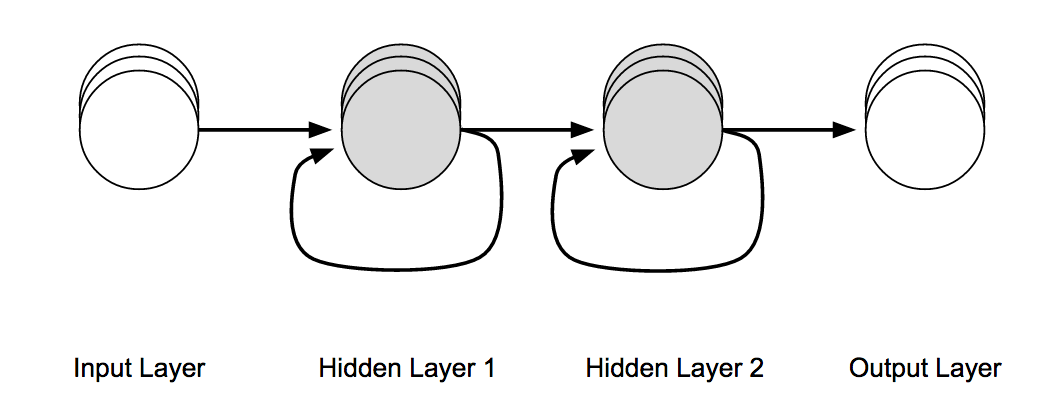
\includegraphics{Images/rnnrolled.png}
\caption{Recurrent connections between the hidden layers of a network}
\end{figure}

\begin{figure}
\centering
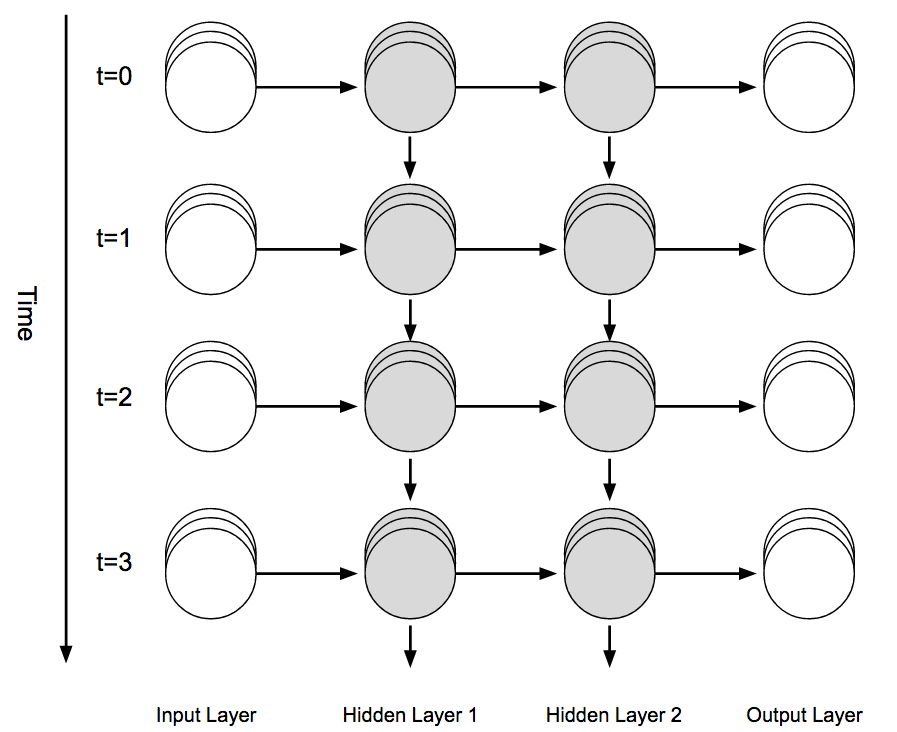
\includegraphics{Images/rnnunrolled.png}
\caption{Identical to the previous figure but with the recurrent
connections unrolled along the time axis}
\end{figure}

\hypertarget{lstms}{%
\subsubsection{LSTMs}\label{lstms}}

\hypertarget{grus}{%
\subsubsection{GRUs}\label{grus}}

\hypertarget{dilation}{%
\subsection{Dilation}\label{dilation}}

The concept of dilation was first proposed in the context of
convolutional neural networks
{[}\protect\hyperlink{ref-yu2015multi}{6}{]} for image analysis and
semantic segmentation; this work was discovered during research for a
\protect\hyperlink{sentimentfromimages}{potential extension} of this
project. The main concept is to aggregate information at different
contextual scalings without losing resolution by exploding a kernel's
considered neighbourhood around a central pixel / element. This is done
to increase the likelihood of discovering pattern structures at
different resolutions within an input as well as increasing the area of
an image or input which can be considered through a small number of
steps.

It offers an alternative to other techniques often relying on
down-sampling which sacrifice resolution rather than considering
different contexts at full resolution as is the case with dilation.

\begin{figure}
\centering
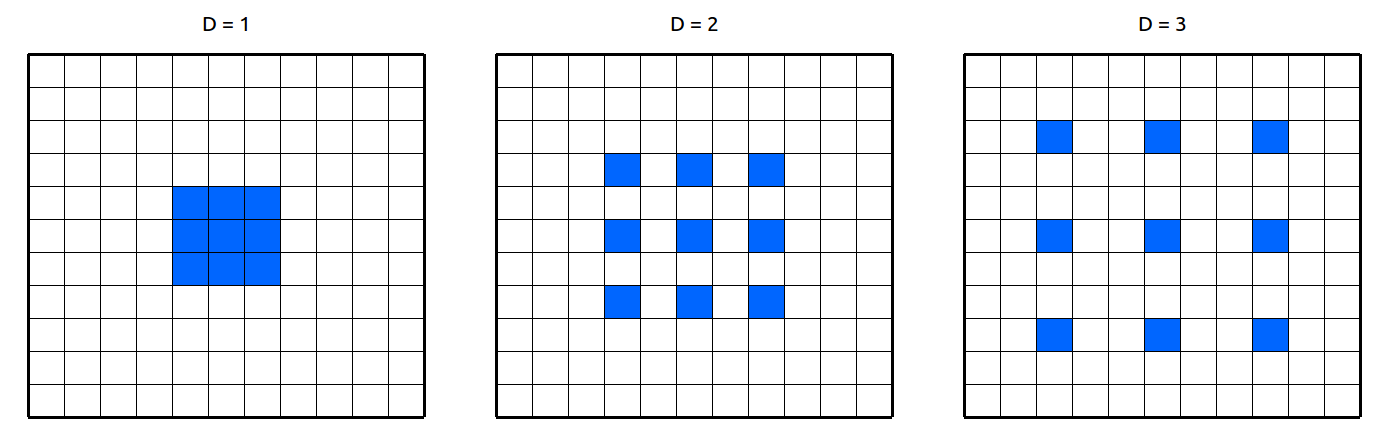
\includegraphics{Images/dilationconv2.png}
\caption{Different dilation factors (represented by the value of D)
illustrated on a 2-dimensional input}
\end{figure}

This technique has shown to be very effective in aiding dense prediction
problems (predicting labels for each pixel in an image, or with respect
to this project's proposed equivalence of predicting on or off states
for each note on the piano over a series of time steps). Deepmind
researchers applied a similar approach within their own convolutional
network for WaveNet which is the first documented use of dilation in the
musical composition domain
{[}\protect\hyperlink{ref-oord2016wavenet}{7}{]}. Their results found
that again the addition of dilation conceptually increased the accuracy
and effectiveness of their model.

A paper was published linking this concept with recurrent neural
networks in 2017 by Chang et
al.~{[}\protect\hyperlink{ref-chang2017dilated}{8}{]}. This paper forms
the basis for the justification of using dilation in the model present
in this project; this project's compositional model is potentially the
first use of dilated recurrent neural networks in the musical
composition domain.

\begin{figure}
\centering
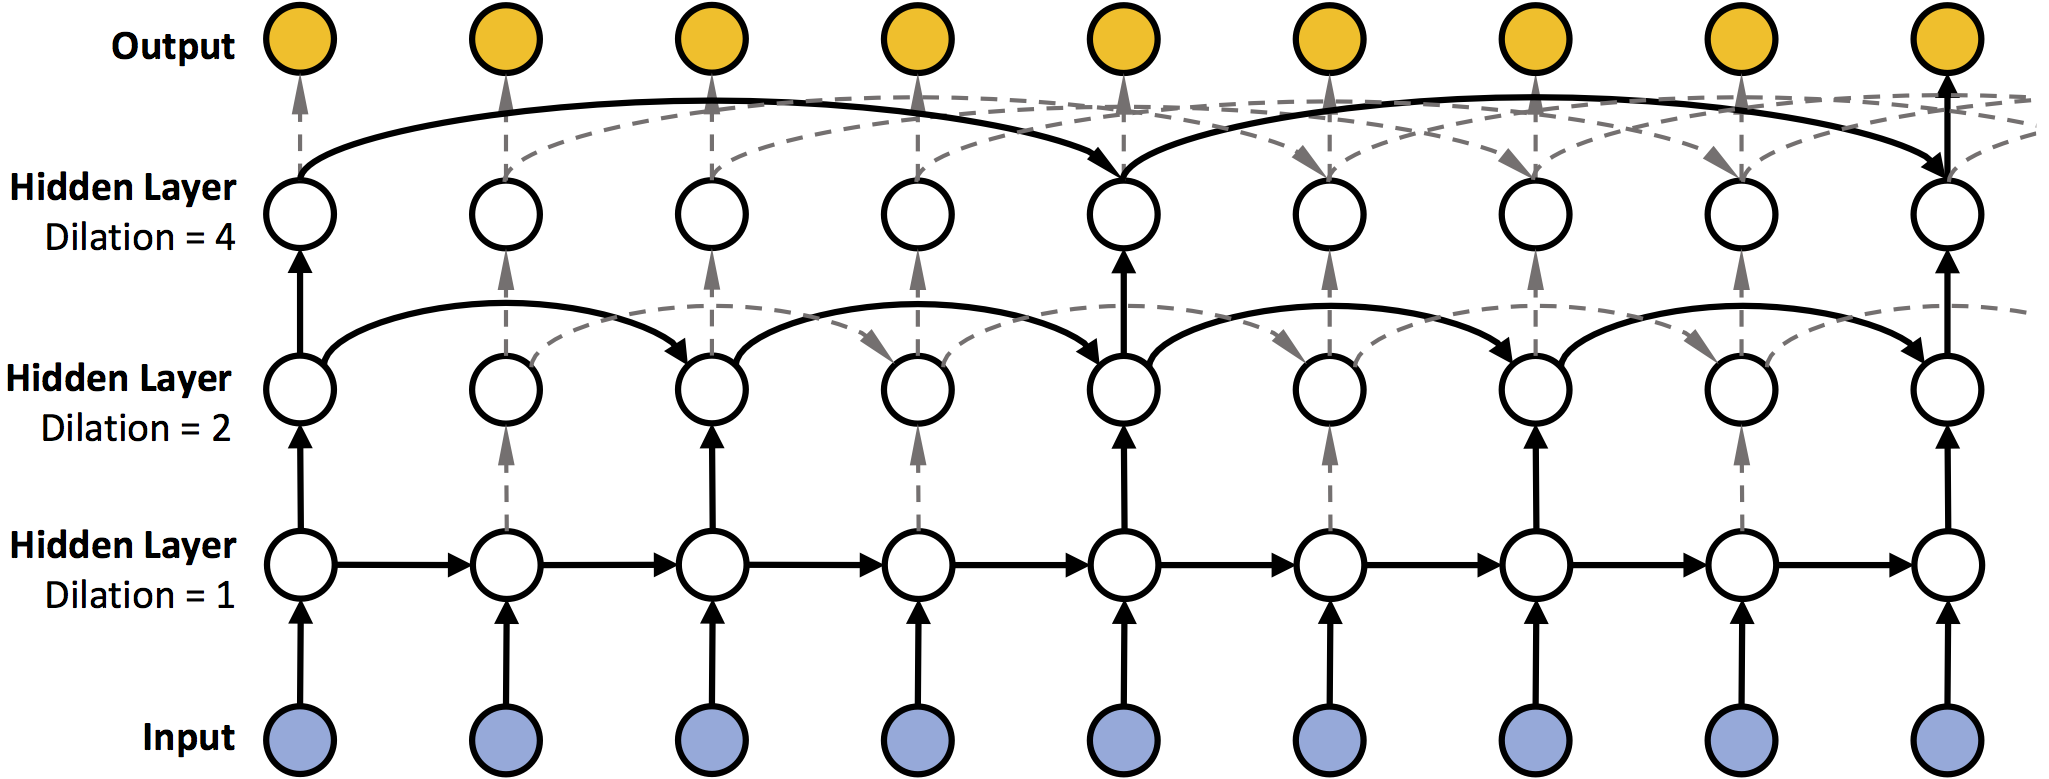
\includegraphics{Images/dilationrnn.png}
\caption{An example of a three-layer DRNN with dilation factors 1, 2,
and 4}
\end{figure}

\hypertarget{related-work}{%
\subsection{Related Work}\label{related-work}}

\begin{enumerate}
\def\labelenumi{\arabic{enumi}.}
\setcounter{enumi}{3}
\item
  RNNs despite their invariance lack long term coherence meaning they
  often fail when complex dependencies are built up and different
  temporal structures must be captured. To combat these issues Long
  short term memory networks, dilated RNNs, restricted Boltzmann
  Machines etc have been developed. They all model joint distributions
  or conditional probabilities like RNNs but involve mechanisms to
  ensure a greater understanding of long term structure in the models.
  The greatest issue with RNNs in this area is their tendency towards
  exploding or vanishing gradients over time due to repeated and
  recurrent backpropagation, i.e.~tiny values will often compound and be
  multiplied together leading to the network getting stuck or learn very
  slowly. All of these variants minimise these problems in various ways
  and so lend themselves better to creating structured, coherent outputs
  like music.
\item
  Image processing has some parallels to my approach as well. I wanted
  to introduce more concepts of relativity into my model over absolute
  structures beyond just the time thing; many existing solutions include
  networks where each note corresponds to a specific node. However,
  music is more of a relative set of rules in that pieces can be
  transposed up or down in key and you can always construct chords and
  melodies relative to that key. So I wanted my network to be able to
  capture this understanding rather than just being able to copy certain
  chords it learns; this way it can perform in a more varied and
  realistic way. Image processing has a similar idea already in which a
  kernel is used to take a neighbourhood of pixels in an image and carry
  out some transformation on them. My idea was to do this with an octave
  above and below each note, feeding this neighbourhood into its own
  network which would then focus only on the relative position of notes
  to learn harmonic structure without worrying which note was actually
  being played.
\end{enumerate}

\hypertarget{competitive-existing-solutions}{%
\subsubsection{Competitive Existing
Solutions}\label{competitive-existing-solutions}}

In terms of a symbolic approach (something that was not considered due
to lack of training data, using musical scoring in terms of sheet music,
lettering representing notes), one of the most impressive was undertaken
by Sturm et al.~from the KTH Royal Institute of Technology and Kingston
University in producing a full album with trained musicians and having
it reviewed without revealing the nature of its composition. This is a
very effective but resource intensive means of qualitative assessment as
well as an effective example of a Turing Test for computational
composition tasks.

Following on from the questions posed in the Specification, a great deal
of research has been carried out in order to better define the
associated objectives. Resolutions to most of these questions have been
reached following testing or further research, and implementations have
been attempted where appropriate in order to properly compare the
options outlined previously. Balance in terms of resources required and
complexity of the task were the main considerations throughout this
process, leading to a realistic but challenging set of goals for the
future.

\hypertarget{transcription-and-encoding-techniques}{%
\subsubsection{Transcription and Encoding
Techniques}\label{transcription-and-encoding-techniques}}

The first objective in the composition section of the Specification
stated that a decision must be made regarding the format of data used to
train the eventual compositional engine. The goal is to build a large
library of this data with enough engineered features for the model to
successfully produce meaningful output. It has become clear that the use
of raw audio data involves a much larger computational overhead making
it an infeasible approach given the time-scale of this project. This
decision will be discussed at greater length
\protect\hyperlink{neuralnetworkapproach}{in the appropriate section};
in terms of encoding input data, the decision is mainly based upon the
large body of existing research behind MIDI transcription and the
intuitiveness of features which arise from relatively simple data such
as this. Characteristics such as tempo can be extracted easily and used
to train a model on the fundamental `rules' of music, from which the
model can then learn to improvise and compose within certain
constraints.

Ableton (a company at the forefront of digital audio technology)
employee Anna Wszeborowska spoke at EuroPython 2016 on the applications
of Python in encoding from raw audio data to MIDI
{[}\protect\hyperlink{ref-annaw}{9}{]}. Indeed, an implementation to
this end has been partially completed, producing some interesting
results. Google Brain's Magenta was heralded in the specification as one
of the more promising existing tools: a TensorFlow sub-package focussing
on musical composition, transcription and other artistic endeavours. The
`Onset Frames' model
{[}\protect\hyperlink{ref-magentaonsetframes}{10}{]} from Magenta's
library of pre-trained models uses Neural Networks to transcribe piano
pieces to MIDI, and also works reasonably well in transcribing other
forms of music.

Cross-validation between this model's output and a method of encoding
raw audio to MIDI implemented in Python will be attempted as both
approaches have shown themselves to be successful; often one is better
than the other depending on the structure of the source. `Onset Frames'
is clearly optimal in the situations it was designed for, whilst
implementations attempted in Python give mixed results that are more
consistent across different styles of music. The biggest challenges
encountered in this part of the project are complex sequences of chords
and polyphony in the input from different instruments and vocals. Both
of the above techniques can deal with these challenges, but with a
slightly lower accuracy than quick successions of monophonic notes for
example.

Another option which is yet to be considered is the use of Convolutional
Neural Networks. These have been applied extensively in the past to the
task of musical transcription
{[}\protect\hyperlink{ref-bereketai}{11}{]}--{[}\protect\hyperlink{ref-sigtia2016end}{13}{]}
with state-of-the-art results at their resolutions. It is likely that as
the project progresses, work on applying this existing research and
exploration into the possibilities of other models will continue and be
refined to best match the desired output of training data to be used as
inputs for the compositional engine. This process exemplifies one of the
largest challenges and complexities in this project: using machine
learning to \emph{generate} the data used to then compose music in a
similar way introduces a lot of uncertainty and dependence between these
two components.

\hypertarget{data}{%
\subsubsection{Data}\label{data}}

All of the approaches to transcription are impractical to a certain
extent following on from the concerns regarding time requirements and
uncertainty made above; it is for this reason that some large MIDI data
libraries such as the Lakh dataset
{[}\protect\hyperlink{ref-lakh}{14}{]} and Metacreation's corpus
{[}\protect\hyperlink{ref-metacreation}{15}{]} could still be fallen
back on if time becomes too constrictive. The existence of such datasets
allows for work on the compositional engine to begin without delay, but
ideally one of the approaches above will eventually lead to the creation
of a similar dataset to be utilised in more intricate feature
engineering as well as being a more relevant dataset to the genres of
music which comprise the initial focus of this project. The MAESTRO Data
Set of MIDI corresponding to piano transcriptions
{[}\protect\hyperlink{ref-maestro2018}{16}{]} is used by Magenta to
train their Onset Frames model and so could also form part of the
training data for the project.

MIDI is easy to work with and clear in its structure, especially when
compared to the complexities of raw audio waveform data. However, there
is still the matter of actually using this data to train a model; for
this TensorFlow already has a technique for converting MIDI to so-called
`Note Sequences' {[}\protect\hyperlink{ref-notesequences}{17}{]} which
define all the characteristics of a MIDI file in a Pythonic format. This
conversion is painless and allows for more standard feature engineering
and manipulation techniques to be done inside of Python using familiar
packages.

\hypertarget{composition}{%
\subsection{Composition}\label{composition}}

\hypertarget{markovian-approach}{%
\subsubsection{Markovian Approach}\label{markovian-approach}}

This approach involved implementing a learned state-space based upon
interpolations of a series of MIDI files. Markov chains could then be
implemented to traverse this state-space and sequentially generate new
MIDI, building compositions from probabilistic sequences of notes. The
idea was to have an `improvisational' algorithm which could
stochastically traverse common progressions and chords, incorporating
the ability to switch between these sequences and build a more complex
overall piece. Initial work on this approach provided a clear-cut first
step to the project as it did not require a huge amount of prior work
due to familiarity with the mechanisms and concepts behind it, as well
as the existence of other attempts at Markovian composition
{[}\protect\hyperlink{ref-markovcomposer}{18}{]}.

The ease of this approach also summarises its main disadvantage: there
is a noticeable lack of complexity and novelty in the pieces composed.
By its nature, most of the states which the composer can traverse are
directly influenced by the input data and thus often lead to sections
which are identical to one of the inputs. This could be attributed to a
lack of training data, though using more lead to increasingly small
transition probabilities and a descent into near randomness, losing a
lot of the musicality present in previous outputs along the way.

It is unlikely that this approach will be revisited and although some
output was generated, it was not particularly impressive and certainly
pales in comparison to some of the witnessed outputs generated by other
techniques. It is for this reason that the second of the big objective
questions in the Specification could be answered, concluding that Neural
Networks should be used for composition rather than Markov Chains.

\hypertarget{neural-network-approach}{%
\subsubsection{Neural Network Approach}\label{neural-network-approach}}

These are recurrent neural networks which most importantly for my
application have the property of time invariance, in that at a given
time step the networks activations and learned properties can all be
considered relative to previous time states. The outputs at one time
step become inputs for the next and we can use this to sequentially
train and generate music without worrying about specific locations or
times within the network. To offer a counter example that might make
this clearer I would imagine a network composed of a fixed sequence of
layers which are visited once and then output to the next layer, dealing
with absolute positions would make this kind of network unsuitable for
musical composition.

Neural Networks are undoubtedly a very active area of research; a lot of
which is relevant or could even be directly applied to this project. For
example, ``How we Made Music Using Neural Networks''
{[}\protect\hyperlink{ref-alextavgen}{19}{]} references an article by
Andrej Karpathy (Tesla's Director of AI); both of these pieces together
formulate a good introduction to the technologies to be implemented for
a large portion of the remainder of this project. The Karpathy article
{[}\protect\hyperlink{ref-karpathy}{20}{]} showcases some of the
capabilities of Recurrent Neural Networks working on generating code,
text and images. Music is considered to be a more challenging feat for
these systems, which is perhaps intuitive given its continuous and often
chaotic nature. The former of the two articles discusses a short
exploration into this challenge, a challenge which this project will go
further in trying to tackle.

Google's Magenta project was mentioned as one of the main leads for
composition in the specification and remains so at this point in the
project. Magenta's collection of pre-trained models is testament to the
promise of this platform; more specifically there are pre-trained models
available which produce improvisation, polyphony and interpolation of
input pieces {[}\protect\hyperlink{ref-magentavae}{21}{]},
{[}\protect\hyperlink{ref-magentapolyphony}{22}{]}. The aim of this
project is to build and train a model sitting somewhere between these
existing ones, one which is capable of generating inspired sequences of
chords and notes and then recurrently feeding these generations back
into itself in order to emulate improvisation.

Based on Magenta's current capabilities, an improvisational RNN
{[}\protect\hyperlink{ref-magentaimprov}{23}{]} combined with an LSTM
net to improvise off interpolations between existing sources would
introduce enough variance and novelty to achieve the goals set for the
compositional engine. Preliminary experiments and tests with the models
are satisfactory for this application; there are a plethora of provided
Jupyter Notebooks to test out the models and interaction is also
possible through a command line interface. RNNs are likely to suffer
with a lack of global structure, but work well in terms of identifying
characteristics of an input and continuing to improvise, in this case.
An LSTM would be able to maintain awareness of musical features such as
bars, phrases and tempo which should lead to a more acceptable musical
output. Hidden layer activations could be used in an RNN to `remember'
what it is doing and where it may be in a musical phrase. However, it is
yet to be seen how effective this memory will be in practice.

Considering the work done by Magenta's team and prior explorations into
the field by other researchers leads to the conclusion that Neural
Networks show more promise for composition than the Markovian approach.
This choice links back into the choices made for the format of data to
be used to train the models. There are Neural Network based systems
which generate MIDI such as Magenta and DeepJazz
{[}\protect\hyperlink{ref-deepjazz}{24}{]}, in contrast to some which
instead generate raw audio waveforms such as WaveNet, GRUV and SampleRNN
{[}\protect\hyperlink{ref-oord2016wavenet}{7}{]},
{[}\protect\hyperlink{ref-Nayebi2015GRUVA}{25}{]},
{[}\protect\hyperlink{ref-mehri2016samplernn}{26}{]}. As mentioned
previously, using raw audio would be infeasible in a project of this
scale and so a lot of the tools and options for composition with Neural
Networks could immediately be discarded. The outputs from these other
approaches were often more abstract as they were not limited to standard
musical notation enforced by MIDI, for example notes would often merge
into one another without an initial point of attack.

After carrying out research into different Neural Network structures and
use-cases, it can be concluded that a Recurrent Neural Network or LSTM
would be the most appropriate implementation for this task due to the
allowance for different lengths of input and output compared to
something like a Convolutional Neural Network which has fixed input and
output sizes. Some very promising work was carried out in studies on
music generation from MIDI datasets
{[}\protect\hyperlink{ref-hilschermusic}{27}{]},
{[}\protect\hyperlink{ref-wyse2018real}{28}{]} which shows the potential
of RNN's for this task. A similar project called DeepJazz was produced
in a hackathon in a matter of hours and also gave very promising
results, again using an RNN.

\hypertarget{user-input-and-interface}{%
\subsection{User Input and Interface}\label{user-input-and-interface}}

This component of the project is relatively simple and thus has not been
given a great deal of consideration at this stage. A Neural Network
approach to image analysis similar to the one described above would
allow for the definition of features and characteristics required for
the model to gain an understanding of sentiment in music. This could be
achieved through labelling and classification of data into different
`moods' or similar groupings which could eventually lead to it matching
an input's perceived mood with the type of output it creates. The
analysis of images for features is a much simpler task than music; this
area of research is also very active, and many examples of such analysis
can be found on the internet. It is likely that a lot of the theory and
some of the implemented components from the compositional engine could
even be reused in image analysis; although here a CNN would likely be
more appropriate than an RNN due to the stationary nature of image data.

As mentioned briefly in the report, an image as input is not the only
planned way for a user to interact with the compositional engine. It
should also be possible for a user to provide textual input or manually
set parameters which will again influence the compositional engines
output.

\hypertarget{articles-of-interest-in-the-field}{%
\subsection{Articles of Interest in the
Field}\label{articles-of-interest-in-the-field}}

It was clear in the initial stages of this project that the field of
computational musical composition is one of intense and rapid
development, with a lot of the papers cited being from 2015 and later.
Numerous sources of information have been investigated and have proved
conducive in terms of inspiration moving forward with the project. For
example, the research and updates to Google Brain Team's Magenta Blog
{[}\protect\hyperlink{ref-magenta}{2}{]} have been of great interest
throughout the project's development so far as there is a lot of
objective overlap.

The general discussion in this blog alongside that found in articles on
the internet {[}\protect\hyperlink{ref-mediumkylemcdonald}{4}{]},
{[}\protect\hyperlink{ref-mkofler}{29}{]} helped influence the decision
to pursue more complex Neural Network based approaches to composition.
Both of these cite Markovian techniques as a \emph{starting point} for
this area; something which has quite safely been surpassed in every
respect at this point. An article discussing comparisons of various deep
learning tools for music generation
{[}\protect\hyperlink{ref-asimovinst}{30}{]} was also informative,
highlighting Magenta as a tool of great promise.

Another deep learning tool encountered is GRUV
{[}\protect\hyperlink{ref-nayebi2015gruv}{31}{]}, which was mentioned
earlier as being an approach trained on raw audio data. It has been used
to successfully reproduce some very recognisable snippets of music such
as the `Amen Break' (part of a funk record which has been sampled
countless times in popular music) from a set of training data, as well
as producing individual instrument sounds
{[}\protect\hyperlink{ref-fiala}{32}{]}. The reproduction of individual
instruments could lead to an alternative approach to synthesis and
production; layering generated sounds on top of a MIDI composition would
be an interesting challenge if the different instruments could somehow
be associated with sentiment.

\hypertarget{methodology}{%
\section{Methodology}\label{methodology}}

\hypertarget{research-methodology}{%
\subsection{Research Methodology}\label{research-methodology}}

\hypertarget{project-management}{%
\subsection{Project Management}\label{project-management}}

Agile in places, refer to the initial posed questions and answer them to
iteratively come up with a novel and effective approach supported by
research and assessment.

PROJECT DEVELOPMENT this is more about the questions posed and how the
project crystallised over time.

Meetings for advice and aid in resolving some of the key issues in the
project have taken place roughly once or twice per week with the
project's supervisor. This is planned to continue, with the meetings
likely to increase in frequency due to a much lower external workload in
the next academic term.

With most of the preliminary and supporting research complete, as well
as the main few directional questions answered, development may continue
in earnest. Below is an updated Gantt chart to show how the project's
trajectory and schedule has changed since the initial specification, as
well as showing confirmation of the completion of some of the defined
tasks. There are some slight changes following the issues or decisions
discussed earlier in the document, but for the most part the schedule
remains unchanged.

\begin{figure}
\centering
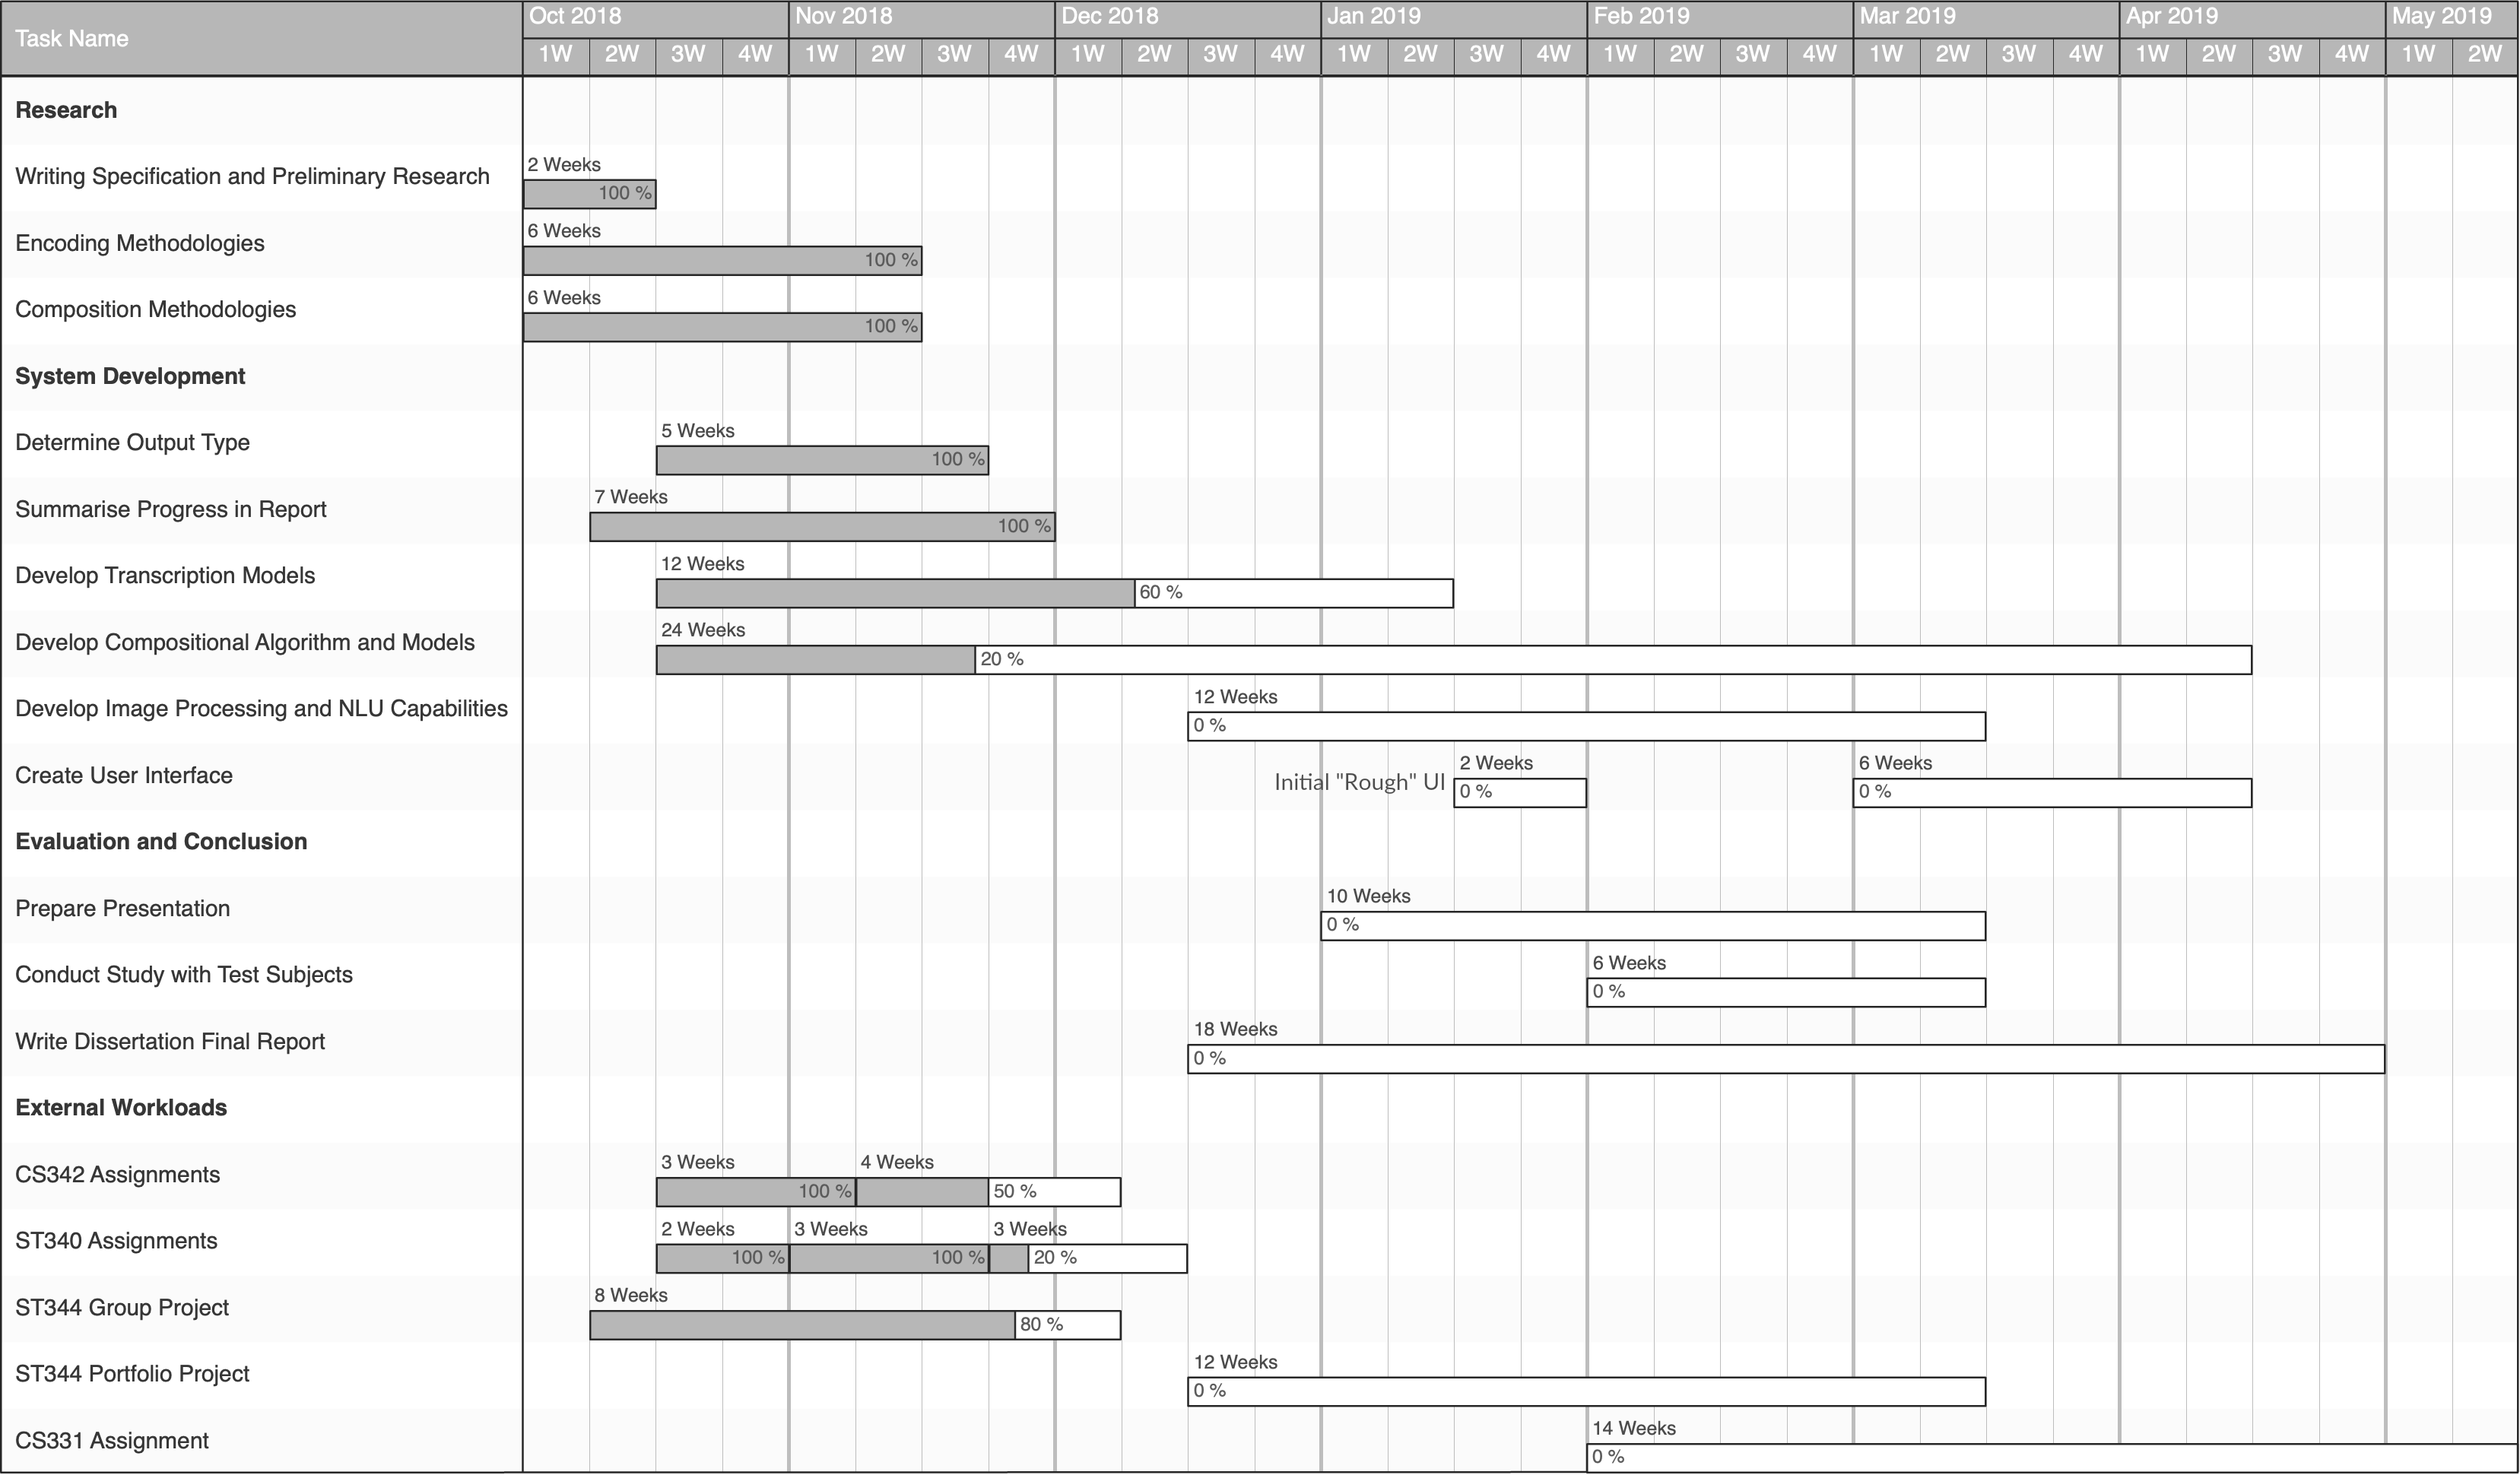
\includegraphics{diss_gantt.png}
\caption{Updated Scheduling Gantt Chart}
\end{figure}

\hypertarget{development-methodology}{%
\subsection{Development Methodology}\label{development-methodology}}

DEVELOPMENT actual programming was iterative combined with agile I
guess, rushed to MVP in order to gain better idea of foreign concepts.

\hypertarget{ethical-considerations}{%
\subsection{Ethical Considerations}\label{ethical-considerations}}

All of the software and projects mentioned so far are freely available
and open source - with the exception of Melodyne - meaning there are no
issues in terms of re-use or forking code for the purposes of this
project. Similarly, the use of any of the datasets mentioned above falls
within the relevant fair-use laws.

It would still be desirable to carry out a survey with some test
subjects to gain qualitative and unbiased assessment of the finished
system. However, given the time constraints and nature of the project
this is not considered critical as there are plenty of other, less
time-consuming means of assessing the outcomes.

\hypertarget{technical-component}{%
\section{Technical Component}\label{technical-component}}

\hypertarget{midi-transcription}{%
\subsection{MIDI Transcription}\label{midi-transcription}}

In order to determine which MIDI transcriptions were best, a number of
factors were considered. Some preliminary testing was done by first
designing a sequence of MIDI notes which could then be played internally
and exported as an audio file. These MIDI notes acted as a ground truth.
Within these test files, chords and complex structures were included as
well as different levels of white noise applied to them. From here
different techniques could be tried in order to decide which would be
best:

\begin{itemize}
\tightlist
\item
  WaoN {\textbf{???}} is a transcription tool which converts
  \texttt{.wav} audio files to \texttt{.midi} files. It carries out
  frequency-domain analysis using Fast Fourier Transforms which are
  computationally intensive but are flexible and accurate when compared
  to simpler autocorrelational techniques {[}klapuri2004automatic;
  gerhard2003pitch{]} meaning they are often applied to more complex
  tasks such as pulling out polyphonic features in music as was the goal
  of this part of the project. This technique requires no training data
  and so can be quickly applied to a large array of audio; it is not
  restricted to a specific genre according to its creator and even has
  means to try and remove drum sounds when transcribing.
\item
  Magenta's `Onset Frames' model
  {[}\protect\hyperlink{ref-magentaonsetframes}{10}{]} is considered
  cutting edge and utilises a convolutional recurrent neural network
  architecture to predicts pitch events both in a framewise and onset
  context. I.e. it first predicts where notes may begin and then uses
  these predictions to influence predicted frames where a certain pitch
  is present. Where these predictions are in agreement (an onset is
  predicted for that pitch within the predicted pitch frame) a note is
  presumed to be present and can be transcribed to MIDI. Training data
  and scope again rears its head as an issue with this approach, as is
  mentioned in the referenced paper.
\end{itemize}

Based on the transcriptions both create it is possible to compare them
qualitatively. Magenta's approach is decisive in its choice of notes and
often more confident when it comes to timing due to its training
instilling a greater sense of tempo and structure in its transcriptions.
WaoN is delicate and plays with wide dynamic range, but often
incorporates more false positives in terms of ghost notes (notes that
should not be present but are determined to be through frequency
clashes, overtones etc.). Both seemed to be viable and offered slightly
different versions of the training data to be used in training the
compositional engine, and as both were viable it was decided that both
should be used. Magenta's model shows great promise and it is likely
that with the correct training data this approach would be far superior
to WaoN in fixed domain transcriptions (i.e.~training the model on a
dataset of ground truth transcriptions of a certain genre before using
it to transcribe more of that genre, so that it might understand the
`rules' of transcribing genres other than classical more effectively). I
have no doubt that in the next few years applications such as WaoN will
be largely eschewed in favour of modern machine learning approaches
similar to what has happened to the field of Computer Vision over the
past decade or so.

\hypertarget{the-model}{%
\subsection{The Model}\label{the-model}}

\hypertarget{dilation-1}{%
\subsubsection{Dilation}\label{dilation-1}}

\hypertarget{design}{%
\subsection{Design}\label{design}}

\hypertarget{implementation}{%
\subsection{Implementation}\label{implementation}}

\hypertarget{theory-1}{%
\subsection{Theory}\label{theory-1}}

\hypertarget{testing}{%
\subsection{Testing}\label{testing}}

Functional testing, unit testing, integration testing ? testing
strategies

\hypertarget{evaluation}{%
\section{Evaluation}\label{evaluation}}

\hypertarget{conclusions}{%
\subsection{Conclusions}\label{conclusions}}

A favourable configuration was found though further investigation would
be required. The function aimed for is a complex one and it is still
somewhat unclear how many neurons might work best in modelling the full
potential. Here resources of time and computational power must be
considered.

\hypertarget{internal-comparison-of-work}{%
\subsection{Internal Comparison of
Work}\label{internal-comparison-of-work}}

\hypertarget{contextualised-comparisons-with-existing-solutions}{%
\subsection{Contextualised Comparisons with Existing
Solutions}\label{contextualised-comparisons-with-existing-solutions}}

\hypertarget{future-work}{%
\subsection{Future Work}\label{future-work}}

As has already been alluded to, experimentation with larger corpuses of
data would be an interesting and engaging extension of this work.

Look into SRUs would be cool, potential improvement over GRUs, moving
averages present potential relevance to music as a format.

\hypertarget{performance-and-interactivity}{%
\subsubsection{Performance and
Interactivity}\label{performance-and-interactivity}}

One of the most interesting extensions of this project would be to
enable the most obvious and intuitive \emph{application} of it. A means
of performance or interactivity would be desirable given the chance;
Magenta again could be used for this with its MIDI Interface
{[}\protect\hyperlink{ref-magentamidi}{33}{]}, allowing for the use of a
virtualised MIDI Controller called VMPK
{[}\protect\hyperlink{ref-vmpk}{34}{]} and Software Synthesiser
FluidSynth {[}\protect\hyperlink{ref-fluidsynth}{35}{]}.

The default purpose of the MIDI Interface is to allow for a user to play
a duet with the computer. In the context of this project, it could allow
a user to give the compositional engine some initial inspiration or
guidance and then allow it to compose as it would based upon the usual
inputs.

\hypertarget{synthesiser-parameters}{%
\subsubsection{Synthesiser Parameters}\label{synthesiser-parameters}}

Other researchers have successfully trained a model to change parameters
of a synthesiser during live performance based on a musician's input and
learned preferences {[}\protect\hyperlink{ref-sommer2014towards}{36}{]}.
Moving forward this would be an excellent way to add another dimension
to the project's outputted music; existing studies into the sentiments
behind different timbres and urgency or latency introduced by
manipulations of note attack-delay-sustain-release parameters could form
a basis of some quantitative assessment of the results. The input could
again influence the output through affecting the choice of parameter
programming for the synthesiser used to play the compositions the system
produces.

One of the limitations in choosing to train a model on MIDI as mentioned
earlier is that the output is also somewhat restricted to this format.
At which point choices could be made in terms of how this MIDI is
synthesised and played back to the user. This could range from something
as simple as instrumental selection, to the tuning of parameters of a
chosen synthesis engine as described here.

\hypertarget{authors-assessment-of-the-project}{%
\subsection{Author's Assessment of the
Project}\label{authors-assessment-of-the-project}}

The work discussed indicates the level of technical achievement this
project encompasses. Much of the work is of a high level for a third
year project and involved significant time investment to learn
additional advanced material with which to accomplish the goals of the
project.

The use of neural networks and deep learning is adherent to the
description of my degree; probablistic sequence generation is certainly
relevant in almost all aspects to the statistical and computational
nature of the BSc in Data Science. The project illustrates domain
knowledge spanning multiple fields relevant to data science and involved
numerous challenging components from a research, theoretical, technical
and engineering perspective.

It is hoped that this work forms a relatively robust and
all-encompassing summary of not only the outputs of the project but the
work involved in achieving it. Other academics and students will
hopefully find value in this work and be able to continue to contribute
to this fast-moving field. Musical composition as mentioned is a
sufficiently complex task to fully leverage some of the more advanced
deep learning and sequential modelling techniques which are currently of
interest in academia; this work shows their potential applications as
well as hopefully contributing to their further development.

Why should this project be considered an achievement?

The incorporation of mood is perhaps the initial limitation an observer
may encounter in terms of the initial goals of the project.

\hypertarget{references}{%
\section*{References}\label{references}}
\addcontentsline{toc}{section}{References}

\hypertarget{refs}{}
\leavevmode\hypertarget{ref-eck2002finding}{}%
{[}1{]} D. Eck and J. Schmidhuber, ``Finding temporal structure in
music: Blues improvisation with lstm recurrent networks,'' in
\emph{Proceedings of the 12th ieee workshop on neural networks for
signal processing}, 2002, pp. 747--756.

\leavevmode\hypertarget{ref-magenta}{}%
{[}2{]} \relax Google Brain Team, ``TensorFlow Magenta.'' \\
\url{https://github.com/tensorflow/magenta}.

\leavevmode\hypertarget{ref-huang2018improved}{}%
{[}3{]} C.-Z. A. Huang \emph{et al.}, ``An improved relative
self-attention mechanism for transformer with application to music
generation,'' \emph{arXiv preprint arXiv:1809.04281}, 2018.

\leavevmode\hypertarget{ref-mediumkylemcdonald}{}%
{[}4{]} K. McDonald, ``Neural nets for generating music.'' \\
\url{https://medium.com/artists-and-machine-intelligence/neural-nets-for-generating-music-f46dffac21c0}.

\leavevmode\hypertarget{ref-libdlmusic}{}%
{[}5{]} Y. Bayle, ``Deep learning for music chronicle.'' \\
\url{https://github.com/ybayle/awesome-deep-learning-music}.

\leavevmode\hypertarget{ref-yu2015multi}{}%
{[}6{]} F. Yu and V. Koltun, ``Multi-scale context aggregation by
dilated convolutions,'' \emph{arXiv preprint arXiv:1511.07122}, 2015.

\leavevmode\hypertarget{ref-oord2016wavenet}{}%
{[}7{]} A. van den Oord \emph{et al.}, ``WaveNet: A generative model for
raw audio.'' 2016 {[}Online{]}. Available:
\url{http://arxiv.org/abs/1609.03499}

\leavevmode\hypertarget{ref-chang2017dilated}{}%
{[}8{]} S. Chang \emph{et al.}, ``Dilated recurrent neural networks,''
\emph{arXiv preprint arXiv:1710.02224}, 2017.

\leavevmode\hypertarget{ref-annaw}{}%
{[}9{]} A. Wszeborowska, ``Music Transcription with Python.'' \\
\url{https://www.youtube.com/watch?v=9boJ-Ai6QFM\&feature=youtu.be}.

\leavevmode\hypertarget{ref-magentaonsetframes}{}%
{[}10{]} \relax Google Brain Team, ``Magenta - Polyphonic Piano
Transcription.'' \\
\url{https://magenta.tensorflow.org/onsets-frames}.

\leavevmode\hypertarget{ref-bereketai}{}%
{[}11{]} M. Bereket and K. Shi, ``An ai approach to automatic natural
music transcription.''

\leavevmode\hypertarget{ref-mbereket}{}%
{[}12{]} \relax mbereket, ``Music Transcription Repository.'' \\
\url{https://github.com/mbereket/music-transcription}.

\leavevmode\hypertarget{ref-sigtia2016end}{}%
{[}13{]} S. Sigtia, E. Benetos, and S. Dixon, ``An end-to-end neural
network for polyphonic piano music transcription,'' \emph{IEEE/ACM
Transactions on Audio, Speech, and Language Processing}, vol. 24, no. 5,
pp. 927--939, 2016.

\leavevmode\hypertarget{ref-lakh}{}%
{[}14{]} C. Raffel, ``Lakh midi dataset.'' \\
\url{https://colinraffel.com/projects/lmd}.

\leavevmode\hypertarget{ref-metacreation}{}%
{[}15{]} M. Lab, ``Metacreation lab.'' \\
\url{http://metacreation.net/corpus-1/}.

\leavevmode\hypertarget{ref-maestro2018}{}%
{[}16{]} C. Hawthorne \emph{et al.}, ``Enabling factorized piano music
modeling and generation with the maestro dataset,'' \emph{arXiv preprint
arXiv:1810.12247}. 2018.

\leavevmode\hypertarget{ref-notesequences}{}%
{[}17{]} \relax Google Brain Team, ``NoteSequence Conversion Guide.'' \\
\url{https://github.com/tensorflow/magenta/blob/master/magenta/scripts/README.md}.

\leavevmode\hypertarget{ref-markovcomposer}{}%
{[}18{]} \relax anbud, ``Markov composer (java application).'' \\
\url{https://github.com/anbud/MarkovComposer}.

\leavevmode\hypertarget{ref-alextavgen}{}%
{[}19{]} A. Tavgen, ``How we made music using neural networks.'' \\
\url{https://medium.com/@ATavgen/how-we-made-music-using-neural-networks-449a62b8a332}.

\leavevmode\hypertarget{ref-karpathy}{}%
{[}20{]} A. Karpathy, ``The unreasonable effectiveness of recurrent
neural networks.'' \\
\url{http://karpathy.github.io/2015/05/21/rnn-effectiveness/}.

\leavevmode\hypertarget{ref-magentavae}{}%
{[}21{]} \relax Google Brain Team, ``Magenta - Music VAE Model.'' \\
\url{https://github.com/tensorflow/magenta/tree/master/magenta/models/music_vae}.

\leavevmode\hypertarget{ref-magentapolyphony}{}%
{[}22{]} \relax Google Brain Team, ``Magenta - Polyphony RNN Model.'' \\
\url{https://github.com/tensorflow/magenta/tree/master/magenta/models/polyphony_rnn}.

\leavevmode\hypertarget{ref-magentaimprov}{}%
{[}23{]} \relax Google Brain Team, ``Magenta - Improvisational RNN
Model.'' \\
\url{https://github.com/tensorflow/magenta/tree/master/magenta/models/improv_rnn}.

\leavevmode\hypertarget{ref-deepjazz}{}%
{[}24{]} J.-S. Kim, ``DeepJazz.'' \\
\url{https://github.com/jisungk/deepjazz}.

\leavevmode\hypertarget{ref-Nayebi2015GRUVA}{}%
{[}25{]} A. Nayebi and M. Vitelli, ``GRUV : Algorithmic music generation
using recurrent neural networks,'' 2015.

\leavevmode\hypertarget{ref-mehri2016samplernn}{}%
{[}26{]} S. Mehri \emph{et al.}, ``SampleRNN: An unconditional
end-to-end neural audio generation model.'' 2016 {[}Online{]}.
Available: \url{http://arxiv.org/abs/1612.07837}

\leavevmode\hypertarget{ref-hilschermusic}{}%
{[}27{]} M. Hilscher and N. Shahroudi, ``Music generation from midi
datasets.''

\leavevmode\hypertarget{ref-wyse2018real}{}%
{[}28{]} L. Wyse, ``Real-valued parametric conditioning of an rnn for
interactive sound synthesis,'' \emph{arXiv preprint arXiv:1805.10808},
2018.

\leavevmode\hypertarget{ref-mkofler}{}%
{[}29{]} M. Kofler, ``Deep Learning with TensorFlow.'' \\
\url{https://towardsdatascience.com/deep-learning-with-tensorflow-part-3-music-and-text-generation-8a3fbfdc5e9b}.

\leavevmode\hypertarget{ref-asimovinst}{}%
{[}30{]} F. Brinkkemper, ``Analysing Six Deep Learning Tools for Music
Generation.'' \\
\url{http://www.asimovinstitute.org/analyzing-deep-learning-tools-music/}.

\leavevmode\hypertarget{ref-nayebi2015gruv}{}%
{[}31{]} A. Nayebi and M. Vitelli, ``Gruv: Algorithmic music generation
using recurrent neural networks,'' \emph{Course CS224D: Deep Learning
for Natural Language Processing (Stanford)}, 2015.

\leavevmode\hypertarget{ref-fiala}{}%
{[}32{]} \relax Fiala, ``Generating Audio with Deep Learning.'' \\
\url{http://fiala.uk/notes/deep-learning-and-sound-02-generating-audio}.

\leavevmode\hypertarget{ref-magentamidi}{}%
{[}33{]} \relax Google Brain Team, ``Magenta - MIDI I/O.'' \\
\href{https://github.com/tensorflow/magenta/tree/master/magenta/interfaces/midi\%0A}{https://github.com/tensorflow/magenta/tree/master/magenta/interfaces/midi
}.

\leavevmode\hypertarget{ref-vmpk}{}%
{[}34{]} \relax VMPK, ``Software MIDI Controller.'' \\
\url{http://vmpk.sourceforge.net}.

\leavevmode\hypertarget{ref-fluidsynth}{}%
{[}35{]} \relax FluidSynth, ``Software Synthesiser.'' \\
\url{http://www.fluidsynth.org/}.

\leavevmode\hypertarget{ref-sommer2014towards}{}%
{[}36{]} N. Sommer and A. Ralescu, ``Towards a machine learning based
control of musical synthesizers in real-time live performance,'' in
\emph{Proc. Of the 25th modern artificial intelligence and cognitive
science conf., spokane, washington, usa}, 2014, pp. 61--67.


\end{document}
